\section{Vectors in $\mathbb{R}^n$}

\begin{outcome}

\begin{enumerate}
\item[A.] Find the position vector of a point in $\mathbb{R}^n$.
\end{enumerate}
\end{outcome}

The notation $\mathbb{R}^{n}$, where n is a positive integer, refers to the collection of ordered lists of 
$n$ real numbers, that is 
\[
\mathbb{R}^{n} = \left\{ \left( x_{1},\cdots, x_{n}\right)
:x_{j}\in \mathbb{R}\text{ for }j=1,\cdots ,n\right\}
\]
where each $\left( x_{1},\cdots, x_{n}\right)$ is a point of $\mathbb{R}^n$.

In this chapter, we take a closer look at vectors in $\mathbb{R}^n$. First, we will consider what $\mathbb{R}^n$ looks like 
in more detail. Recall that the point given by $0=\left( 0, \cdots, 0 \right)$ is called the \textbf{origin}.

Now, consider the case of $\mathbb{R}^n$ for $n=1.$ Then from the definition we can identify 
$\mathbb{R}$ with points in $\mathbb{R}^{1}$ as follows:
\begin{equation*}
\mathbb{R} = \mathbb{R}^{1}=
 \left\{ \left( x_{1}\right) :x_{1}\in \mathbb{R} \right\}
\end{equation*}
Hence, $\mathbb{R}$ is defined as the set of all real numbers and geometrically,
we can describe this as all the points on a line.

Now suppose $n=2$. Then, from the definition,
\begin{equation*}
\mathbb{R}^{2}=
\left\{ \left(x_{1}, x_{2}\right)
:x_{j}\in \mathbb{R}\text{ for }j=1,2 \right\}
\end{equation*}
Consider the
familiar coordinate plane, with an $x$ axis and a $y$ axis. Any point
within this coordinate plane is identified by where it is located
along the $x$ axis, and also where it is located along the $y$
axis. Consider as an example the following diagram.

\begin{center}
\begin{tikzpicture}
\draw[<->](-4,0)--(4,0);
\draw[<->](0,-1)--(0,5);
\draw(2,0.2)--(2,-0.2);
\draw(-3,0.2)--(-3,-0.2);
\draw(-0.2,1)--(0.2,1);
\draw(-0.2,4)--(0.2,4);
\draw[help lines] (-3,0)--(-3,4)--(0,4);
\draw[help lines](0,1)--(2,1)--(2,0);
\draw[fill=red](-3,4) circle [radius=3pt];
\draw[fill=red](2,1) circle [radius=3pt];
\node[below right] at (4,0){$x$};
\node[left] at(0,5){$y$};
\node[below] at (-3,-0.5){$-3$};
\node[below] at (2,-0.5){$2$};
\node[left] at (-0.5, 1){$1$};
\node[left] at (-0.5, 4){$4$};
\node[above] at (-3,4){$Q = (-3,4)$};
\node[above] at (2,1){$P = (2,1)$};
\end{tikzpicture}
\end{center}

Hence, every element in $\mathbb{R}^2$ is identified by two
components, $x$ and $y$, in the usual manner. The coordinates $x, y$ (or $x_1$,$x_2$) uniquely determine a point in the plan. Note that while the definition uses $x_1$ and $x_2$ to label the coordinates and you may be used to $x$ and $y$, these notations are equivalent. Thus $\mathbb{R}^2$ can be represented by the two-dimensional coordinate plane.

Now suppose $n=3$. You may have previously encountered the $3$-dimensional
coordinate system, given by
\begin{equation*}
\mathbb{R}^{3}=
\left\{ \left( x_{1}, x_{2}, x_{3}\right)
:x_{j}\in \mathbb{R}\text{ for }j=1,2,3 \right\}
\end{equation*}

Points in $\mathbb{R}^3$ will be determined by three
coordinates, often written $\left(x,y,z\right)$ which correspond to the $x$, $y$,
and $z$ axes.  We can think as above that the first two coordinates
determine a point in a plane. The third component determines the
height above or below the plane, depending on whether this number is
positive or negative, and all together this determines a point in
space. You
see that the ordered triples correspond to points in space just as the
ordered pairs correspond to points in a plane and single real numbers
correspond to points on a line.

The idea behind the more general $\mathbb{R}^n$ is that we can extend
these ideas beyond $n = 3.$ This discussion regarding points in $\mathbb{R}^n$ leads into a study of vectors in $\mathbb{R}^n$. While we consider $\mathbb{R}^n$ for all $n$,
we will largely  focus on $n=2,3$ in this section. 

Consider the following definition.

\begin{definition}{The Position Vector}{positionvector}
Let $P=\left( p_{1},\cdots ,p_{n}\right) $ be the coordinates of a
point in $\mathbb{R}^{n}.$ Then the vector $\longvect{0P}$ with its tail at
$0=\left( 0,\cdots ,0\right) $ and its tip at 
$P$ is called the \textbf{position vector}\index{position vector}\index{vector!points and vectors} of the point $P$. 
We write 
\begin{equation*}
\longvect{0P} = \leftB 
\begin{array}{c}
p_{1} \\
\vdots \\
p_{n}
\end{array} \rightB
\end{equation*}
\end{definition}

$\longvect{0P}$ can be interpreted as a set of directions to get from the origin to the point $P$.
For this reason we may write both $P=\left( p_{1},\cdots ,p_{n}\right)  \in \mathbb{R}^{n}$
and  $$\longvect{0P}= \leftB 
\begin{array}{c}
p_{1} \\
\vdots \\
p_{n}
\end{array} \rightB = \leftB p_{1} \cdots p_{n} \rightB^T \in \mathbb{R}^{n}$$ 
Where $\leftB p_{1} \cdots p_{n} \rightB^T$ is used to lighten the text, the superscript $T$ will be explained in more details in a further chapter.

This definition is illustrated in the following picture for the
special case of $\mathbb{R}^{3}$.

\begin{center}
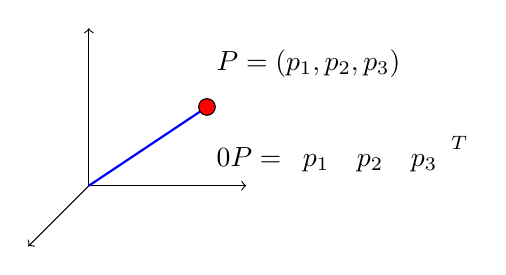
\begin{tikzpicture}
\draw[<->](2,0,0)--(0,0,0)--(0,2,0);
\draw[->](0,0,0)--(0,0,2);
\draw[thick, blue](0,0,0)--(1.5,1,0);
\draw[fill=red] (1.5, 1,0) circle [radius=3pt];
\node[above right] at (1.5, 1.25, 0){$P=(p_1, p_2, p_3)$};
\node[below right] at (1.5, 0.75, 0){$\longvect{0P}= \leftB \begin{array}{ccc}
p_1 & p_2 & p_3 
\end{array}\rightB^T$};
\end{tikzpicture}
\end{center}

Thus every point $P$ in $\mathbb{R}^{n}$ determines its position
vector $\longvect{0P}$. Conversely, every such position vector $\longvect{0P}$
which has its tail at $0$ and point at $P$ determines the point $P$ of
$\mathbb{R}^{n}$.

Now suppose we are given two points, $P,Q$ whose
coordinates are $\left( p_{1},\cdots ,p_{n}\right) $ and $\left(
q_{1},\cdots ,q_{n}\right) $ respectively. We can also determine the
\textbf{position vector from $P$ to $Q$} (also called the \textbf{vector from $P$ to $Q$}) defined as follows.
\begin{equation*}
\longvect{PQ} = \leftB \begin{array}{c}
q_{1}-p_{1}\\
 \vdots \\
q_{n}-p_{n}
\end{array}
\rightB = \longvect{0Q} - \longvect{0P}
\end{equation*}
One can verify that $\longvect{0Q}=\longvect{0P}+\longvect{PQ}$.

Now, imagine taking a vector in $\mathbb{R}^n$ and moving it around, always
keeping it pointing in the same direction as shown in the following picture.

\begin{center}
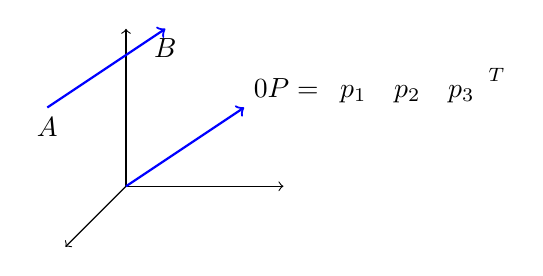
\begin{tikzpicture}
\draw[<->](2,0,0)--(0,0,0)--(0,2,0);
\draw[->](0,0,0)--(0,0,2);
\draw[->, thick, blue](0,0,0)--(1.5,1,0);
\draw[->, thick, blue](-1,1,0)--(0.5,2,0);
\node[right] at (1.5, 1.25, 0){$\longvect{0P}= \leftB \begin{array}{ccc}
p_1 & p_2 & p_3 \end{array}\rightB ^T$};
\node[below] at (-1,1,0){$A$};
\node[below] at (0.5,2,0){$B$};
\end{tikzpicture}
\end{center}

After moving it around, it is regarded as the same vector. On the above picture, both vectors $\longvect{0P}$ and $\longvect{AB}$ have the same length (or magnitude) and direction. Therefore, they are equal, moving a vector in space while preserving its orientation does not alter it.

Consider now the general definition for a vector in $\mathbb{R}^n$. 

\begin{definition}{Vectors in $\mathbb{R}^n$}{vectorsRn}
Let $\mathbb{R}^{n} = \left\{ \left( x_{1}, \cdots, x_{n}\right)
:x_{j}\in \mathbb{R}\text{ for }j=1,\cdots ,n\right\} .$
Then,
\begin{equation*}
\vect{x}
=
\leftB \begin{array}{c}
x_{1} \\
\vdots \\
x_{n}
\end{array}
\rightB 
\end{equation*}
is called a \textbf{vector}\index{vector}. Vectors have both size (magnitude) and direction. 
The numbers $x_{j}$ are called the \textbf{components}\index{vector!components} of $\vect{x}$. 

\end{definition}

Using this notation, we may use $\vect{p}$ to denote the position vector of point $P$. Notice that in this context, $\vect{p} = \longvect{0P}$. These notations may be used interchangeably. 

You can think of the components of a vector as directions for
obtaining the vector. Consider $n=3$.  Draw a vector with its tail at
the point $\left( 0,0,0\right) $ and its tip at the point $\left(
a,b,c\right) $. This vector it is obtained by starting at $\left(
0,0,0\right) $, moving parallel to the $x$ axis to $\left(
a,0,0\right) $ and then from here, moving parallel to the $y$ axis to
$\left( a,b,0\right) $ and finally parallel to the $z$ axis to $\left(
a,b,c\right). $ Observe that the same vector would result if you began
at the point $ \left( d,e,f \right)$, moved parallel to the $x$ axis
to $\left( d+a,e,f\right) ,$ then parallel to the $y$ axis to $\left(
d+a,e+b,f\right) ,$ and finally parallel to the $z$ axis to $\left(
d+a,e+b,f+c\right)$. Here, the vector would have its tail sitting at
the point determined by $A= \left( d,e,f\right) $ and its point at
$B=\left( d+a,e+b,f+c\right)$. It is the \textbf{same vector} because
it will point in the same direction and have the same length. It is
like you took an actual arrow, and moved it from one location to another keeping it pointing
the same direction.\index{vector!addition, geometric meaning}

Notice that two vectors $\vect{u} = \leftB u_{1} \cdots u_{n}\rightB^T $ and
$\vect{v}=\leftB v_{1} \cdots v_{n}\rightB^T$ are equal if and only if
all corresponding components are equal. Precisely,
\begin{equation*}
\begin{array}{c}
\vect{u}=\vect{v} \; \mbox{if and only if}\\
u_{j}=v_{j} \; \mbox{for all}\; j=1,\cdots ,n
\end{array}
\end{equation*} 
Thus 
$\leftB 
\begin{array}{rrr}
1  & 2 & 4
\end{array}
\rightB^T \in \mathbb{R}^{3}$ and $\leftB 
\begin{array}{rrr}
2 & 1 & 4
\end{array}
\rightB^T \in
\mathbb{R}^{3}$ but $\leftB 
\begin{array}{rrr}
1 & 2 & 4
\end{array}
\rightB^T \neq \leftB
\begin{array}{rrr}
2 & 1 & 4
\end{array}
\rightB^T $ because,
even though the same numbers are involved, the order of the numbers is different. 
